\documentclass{hipatia}
\usepackage{lipsum}
%Use \DeclareMathOperator para definir novos
% operadores para o modo matemático
\DeclareMathOperator{\sen}{sen}

%Evite numerar teoremas
%Prefira nomeá-los
%Use os ambientes abaixo
\newtheorem*{theorem*}{Teorema}
\newtheorem*{lemma*}{Lema}

% Evite títulos muito longos
%\title{Uma Nova Demonstração do\\
%Teorema de Pitágoras}
% Se for necessário diminuir a fonte do título 
% para caber no quadro, use
\title{ \fontsize{28}{28}\selectfont Elinalva Vergasta\\  \fontsize{28}{28}\selectfont Afeto, Matemática e Arte}

% O Subtítulo é o nome da seção da revista
% Deve ser uma palavra de origem grega
\subtitle{Biografia}
\author{Dionicarlos Vasconcelos e Elaís Cidely S. Malheiro}
% A data não é necessária
%\date{October 2023}
% Não se preocupe com a numeração
% das páginas ou com o número da edição
\newcommand{\superau}{\textsuperscript{\underline{a}}~}
\newcommand{\superou}{\textsuperscript{\underline{o}}~}

\begin{document}
\setcounter{page}{\biografiapage}
\maketitle

\section{Introdução}
``Treine o cérebro, mas também cultive a compaixão; eduque o intelecto, mas também desperte a
alma.'' \ Inspirado nos ensinamentos de Paramahansa Yogananda, esse princípio --- que valoriza tanto o saber quanto a sensibilidade --- refletia profundamente a atuação da professora Elinalva
Vergasta de Vasconcelos, carinhosamente conhecida como Lina, hoje aposentada pelo Departamento de Matemática da UFBA.

\begin{figure}[htb!]
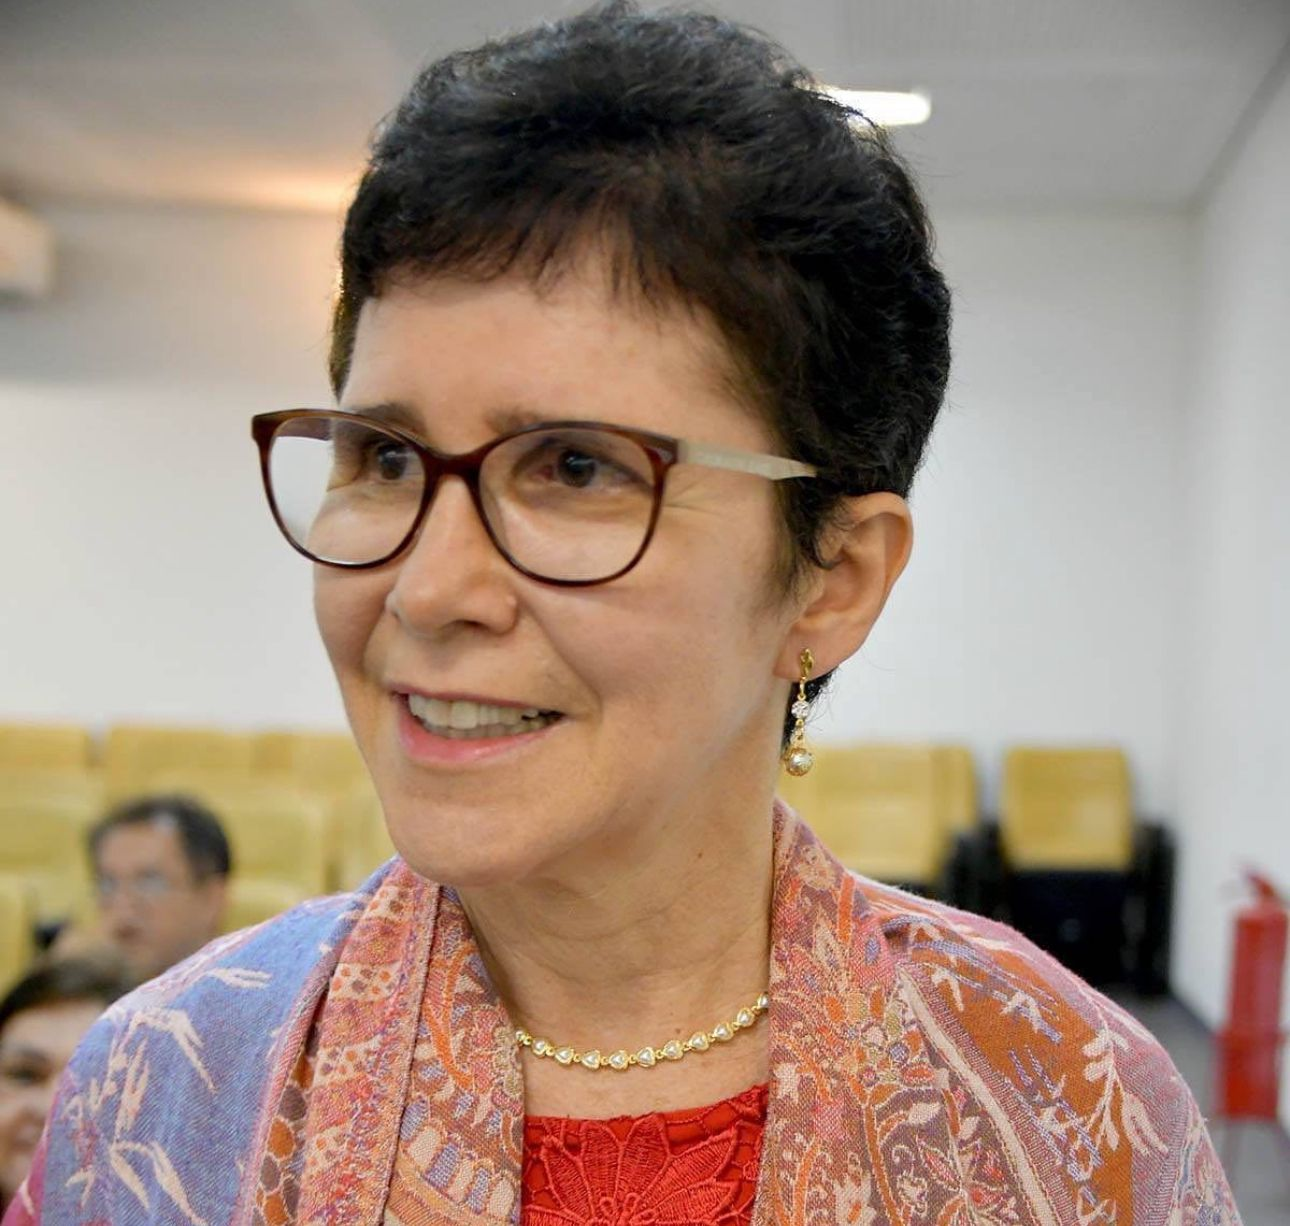
\includegraphics[width=8cm]{Lina.jpg}
\caption{Prof.\superau Lina}   
\end{figure}

Este artigo apresenta uma breve biografia da 
professora Lina, com caráter de celebração e homenagem,
trazendo elementos da sua trajetória e história de vida,
o seu impacto na formação dos estudantes, seu papel 
fundamental na criação e coordenação do 
Laboratório de Ensino de Matemática e Estatística 
da UFBA (LEMA), suas características 
pessoais e profissionais, o reconhecimento que 
conquistou ao longo da carreira, e a maneira 
única com que abordou o ensino da Matemática, 
unindo rigor técnico e afeto.  

Professora Lina foi uma figura extremamente influente e inspiradora na vida de seus alunos e colegas, sempre descrita como uma educadora alegre, dedicada, competente e com uma abordagem inovadora para o ensino da matemática. Seu trabalho no LEMA é amplamente reconhecido como um marco na formação de diversos profissionais, que destacam suas essenciais contribuições para o desenvolvimento acadêmico e humano dos estudantes.  

Muitos alunos e colegas mencionam seu carisma, entusiasmo e a forma como ela transformou o ensino da matemática em algo acessível e motivador. Além disso, sua preocupação com o bem-estar e o crescimento pessoal de seus alunos e colegas é um traço constantemente ressaltado nas conversas com os mesmos. O impacto da professora Elinalva vai além da sala de aula, influenciando carreiras, promovendo projetos inovadores e criando um ambiente acolhedor e inspirador para todos ao seu redor.  

\section{Nasce uma educadora}
Elinalva da Silva Vergasta nasceu em Salvador, no dia 5 de dezembro de 1955. Filha de Eduvaldo Alves Vergasta e Ernestina da Silva Vergasta, cresceu em uma tranquila travessa próxima ao Largo de Roma, onde a paisagem se abria para a Baía de Todos os Santos. Brincava nas areias, jogava futebol na rua em frente de casa, e desde cedo revelava uma personalidade alegre, criativa e generosa. Ainda na infância, começou a participar da Evangelização do Centro Espírita Caminho da Redenção, passando depois à Juventude Espírita Nina Arueira (JENA), onde desenvolvia atividades como teatrinhos de fantoches e sombras para as crianças, e participava de ações sociais, levando mantimentos e carinho a comunidades em situação de vulnerabilidade, além de contribuir na tesouraria do Centro. Costumava ajudar também em casa, ao lado da mãe, demonstrando senso de responsabilidade e cuidado, desde jovem. 


\begin{figure}[htb!]
\includegraphics[width=8cm]{Criança-Lina.jpeg}
\caption{Lina na infância.}   
\end{figure}

O ambiente familiar, cercado por números, teve grande influência em sua trajetória. Seu pai era contador, e tanto sua irmã mais velha quanto seu irmão mais novo cursaram Matemática na UFBA, instituição onde também se graduou o marido, Dionicarlos Vasconcelos, físico de formação. Rodeada por essa atmosfera, Lina escolheu ingressar no Bacharelado em Matemática da UFBA em 1974, ano em que também se casou, passando a se chamar Elinalva Vergasta de Vasconcelos. Apesar da decisão, seu coração guardava um chamado mais artístico. Um teste vocacional feito anteriormente apontava claramente para as artes. Essa veia artística nunca desapareceu: ela se expressava nas interações com crianças, nas brincadeiras, nos jograis e nas dramatizações que encantavam os pequenos e deixavam transparecer sua vocação para ensinar com leveza e criatividade.  

A espiritualidade, por sua vez, esteve sempre presente. Lina não se limitava a uma única crença: era atuante no Centro Espírita, participava de missas e cultos, e em 1973 passou a frequentar o Grupo de Meditação de Salvador, ao lado do seu então namorado Dioni. Aprofundou-se nos ensinamentos de Paramahansa Yogananda, chegando a participar de convocações da Self-Realization Fellowship (SRF) nos Estados Unidos e, em 1998, viajou à Índia para conhecer de perto a espiritualidade daquele país.  

Sobre essas viagens, Cristiana Reis, amiga de Lina da Yoga, lembra com carinho:
\begin{quote} \textit{Conheci Lina no Grupo de Meditação de Salvador - SRF. Durante o tempo em que convivemos, sempre chamou a minha atenção o seu marcante bom humor. Viajei algumas vezes com ela e outros devotos do Grupo, oportunidade em que pude perceber também a sua extraordinária capacidade de lidar com situações adversas e inusitadas. Quando fomos à Índia em 1998, logo no início da viagem, ela quebrou um dente superior. Encarou a situação de forma divertida, leve e continuou a viagem com o seu contagiante bom humor ( e o dentinho colado com "super bonder").}\end{quote}

\begin{figure}[htb!]
\includegraphics[width=8cm]{Casal-Índia.jpg}
\caption{Lina e Dioni na Índia}   
\end{figure}
Mais tarde, como professora universitária e pesquisadora em Geometria Diferencial, encontrou uma maneira de unir todas essas dimensões de sua vida. Passou a construir modelos concretos de superfícies matemáticas, unindo rigor e criatividade, razão e sensibilidade. Dessa fusão nasceu o LEMA – Laboratório de Ensino de Matemática e Estatística da UFBA –, iniciativa que expressa plenamente a educadora que Lina se tornou: uma mulher de números e de alma, que fez da matemática uma linguagem de afeto, beleza e transformação, aliada ao rigor técnico. 
 
\section{Formação, Produção e Atuação}
Sempre se destacando nas disciplinas de Exatas, Elinalva Vergasta iniciou sua formação acadêmica na Escola Castro Alves e, posteriormente, no Colégio Estadual João Florêncio Gomes, na Ribeira. Graduou-se em 1977 como  bacharela em Matemática pela UFBA, mesma instituição na qual, dois anos depois, ingressou no mestrado acadêmico, sob a orientação do professor Dr. Jürgen Tolke. Estando como professor visitante do DMAT, ao precisar retornar à Alemanha, seu país de origem, Tolke deixou Lina sem orientação acadêmica formal por um período. No entanto, sabendo que ele viria ao Brasil, mais especificamente, à cidade de Campina Grande, na Paraíba, Lina se deslocou até lá, acompanhada do esposo, para discutir pontos importantes e encaminhar a finalização da dissertação. Já vegetariana, passou os 15 dias da visita alimentando-se basicamente de sanduíche de queijo e pizza. 

Com a perseverança de sempre, concluiu  sua dissertação na área de Geometria Diferencial, em 1981, sobre Superfícies de Movimento. Neste mesmo ano, iniciou o doutorado no IMPA, onde obteve aprovação em todas as disciplinas, incluindo os intensivos cursos de verão. Porém, a imensa saudade dos filhos, que durante as férias voltavam a Salvador para que ela pudesse se dedicar exclusivamente aos cursos de verão do IMPA, se tornava cada vez mais difícil de conciliar com a demanda acadêmica do doutorado. Tomada pela sensação de que poderia estar sacrificando o bem-estar das crianças, então com 2, 3 e 6 anos de idade, Lina decidiu interromper o doutorado e retornar a Salvador, optando por estar mais presente no cuidado e na criação dos filhos pequenos. Essa escolha, marcada por profundo senso de responsabilidade afetiva, a fez abrir mão do título formal de doutora, mas não do compromisso com a qualidade acadêmica.
Anos depois, um valioso reconhecimento da excelência do seu trabalho foi expresso pelo professor da USP, Ernst Hamburger\footnote{Nascido na Alemanha, o físico Ernst Hamburger deu importantes contribuições ao ensino, pesquisa, divulgação e popularização da ciência. Foi membro da Academia Brasileira de Ciências e, entre outros prêmios no Brasil e no exterior, recebeu o Kalinga Prize for the Popularization of Science, concedido pela UNESCO, em 2000, e o Prêmio José Reis de Divulgação Científica do CNPq. Em 2018, Ernst faleceu, com 85 anos.}, que afirmou, durante visita ao LEMA, que as pesquisas ali desenvolvidas poderiam sustentar não apenas uma, mas várias teses de doutorado na área de Educação Matemática.  

Em busca de aprofundamento e atualização constantes, participou de diversos cursos de formação complementar em instituições, como o Instituto de Matemática Pura e Aplicada (IMPA), a Universidade Federal de São Carlos (UFSCAR), a Universidade Federal do Ceará (UFC) e a própria UFBA. Entre os temas estudados, destacam-se Geometria Riemanniana, Equações Diferenciais Parciais e Ordinárias, Variedades Diferenciáveis, além de cursos voltados ao uso de tecnologias como o Maple V. 


\begin{figure}[htb!]
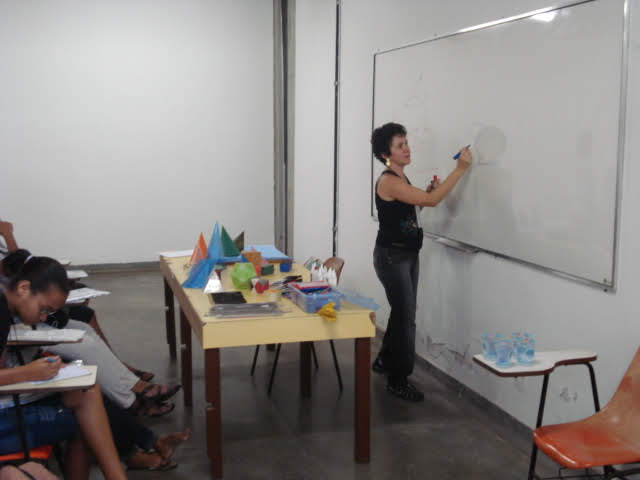
\includegraphics[width=8cm]{Lina em sala de aula.jpg}
\caption{Em sala de aula}   
\end{figure}

Sua atuação como professora do ensino superior teve início na Faculdade de Administração da Bahia (atual UNIFACS), onde lecionou de 1983 a 1984. No final deste período, passou a colaborar com o Instituto de Matemática da UFBA (IM-UFBA), hoje chamado de Instituto de Matemática e Estatística da UFBA (IME-UFBA), instituição na qual construiu uma sólida carreira. Aprovada em concurso público para professora auxiliar em 1994, progrediu para os cargos de professora assistente e, posteriormente, adjunta, alcançando o nível Adjunto IV.  

Como professora do DMAT, lecionou diversas disciplinas, incluindo Cálculo I, II e IV, Geometria Diferencial, Topologia e Álgebra Linear, sempre aliando rigor matemático à sensibilidade pedagógica. Como lembra com carinho a atual coordenadora do LEMA, professora Cristiana Valente(UFBA), em depoimento \footnote{O depoimento completo se encontra na Seção 'Relatos sobre Lina'.} sobre Lina enviado por e-mail aos autores deste artigo: \begin{quote}\textit{Meu contato inicial com Elinalva foi como aluna de Topologia e nas suas aulas ficava encantada como ela apresentava esses conteúdos matemáticos, avançados para graduação, de uma forma tão simples e natural. Nessas aulas tive um choque matemático: ‘uma bola pode ser um quadrado! Tudo depende da maneira de medir’, dizia Elinalva, como se esse fato fosse algo normal....e um novo mundo se abria pra mim.}\end{quote}  
    

\begin{figure}[htb!]
\hspace{2cm}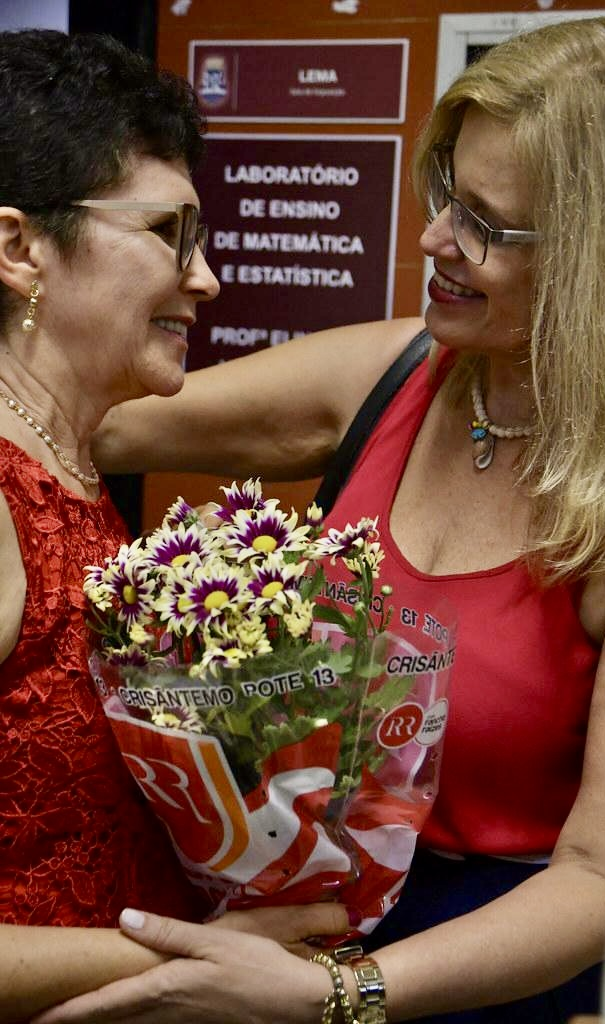
\includegraphics[width=5cm]{Cris.jpg}
\caption{A primeira e a atual coordenadoras do LEMA.}   
\end{figure}


Seu compromisso com a educação pública e de qualidade se expressa também por meio da extensão universitária: Lina coordenou quase 40 projetos de extensão no DMAT, contribuindo diretamente para a democratização do conhecimento matemático e a formação cidadã dos estudantes. Nesse percurso, orientou mais de 50 estudantes de graduação em atividades diversas — de iniciação científica, extensão e ações educativas junto a escolas públicas. Foi ainda responsável por organizar diversos eventos ao longo dos anos, com destaque para as exposições do LEMA e para a coordenação da organização da II Bienal da Sociedade Brasileira de Matemática, eventos marcantes na interface entre matemática, arte e educação.  
 

Além da atuação no ensino, pesquisa e extensão, Lina atuou em diversas atividades administrativas, incluindo a vice-direção do então IM-UFBA e a vice-chefia do DMAT. Requereu sua aposentadoria em 2010, ano em que lançou dois livros pela Editora da UFBA (Edufba): 'Superfícies Isométricas ao Plano – Construção de Modelos Concretos com Cilindros e Cones', em coautoria com Graça Dominguez, Maria Christina Cardoso e Verlane Cabral; e 'Sólidos e Superfícies – Construção de Modelos Concretos', com Ednalva Vergasta Andrade, Maria Christina Cardoso e Maria das Graças Sousa. 

Mesmo após sua aposentadoria, permaneceu intelectualmente ativa e colaborativa. Participou da elaboração de mais uma obra, `Planificação de Pirâmides`, em parceria com Cristiana Valente, Maria Christina Cardoso, Maria das Graças Sousa, Rita de Cássia e Verlane Cabral, demonstrando que seu compromisso com o ensino e a construção de saberes ultrapassava os limites do tempo formal de serviço como professora e educadora.  

Sua produção acadêmica, embora não sempre registrada em periódicos de grande circulação, teve importante impacto na UFBA, especialmente por meio da formação de estudantes, orientação em projetos de iniciação científica e criação de materiais didáticos e modelos concretos de sólidos e superfícies matemáticas. O legado de Elinalva na Educação Matemática é, assim, tanto tangível quanto inspirador.  

Como afirma o professor Kleyber Mota, o atual diretor do IME-UFBA, em relato enviado aos autores: \begin{quote}
   \textit{A trajetória acadêmica e institucional da professora Elinalva é uma referência para todos nós. Ao longo de sua carreira, a professora Elinalva destacou-se pelo compromisso com o ensino de qualidade, pela dedicação à formação de professores e por sua incansável atuação em prol da valorização do ensino de matemática. Sua aposentadoria em 2010 marcou o encerramento de um ciclo brilhante, mas seu legado continua presente no IME e na memória de colegas, alunas e alunos.
Entre suas inúmeras contribuições ao Instituto, merece destaque especial o Laboratório de Ensino de Matemática e Estatística (LEMA). O LEMA, idealizado e estruturado sob sua liderança, tornou-se referência nacional, abrigando projetos que impactaram significativamente a formação de alunos e professores. A professora Elinalva não apenas deixou marcas institucionais profundas, mas também inspirou gerações com sua sensibilidade, competência e compromisso com o ensino de qualidade.} 
\end{quote}


\section{LEMA e o Impacto no ensino e formação de estudantes}

\begin{figure}[htb!]
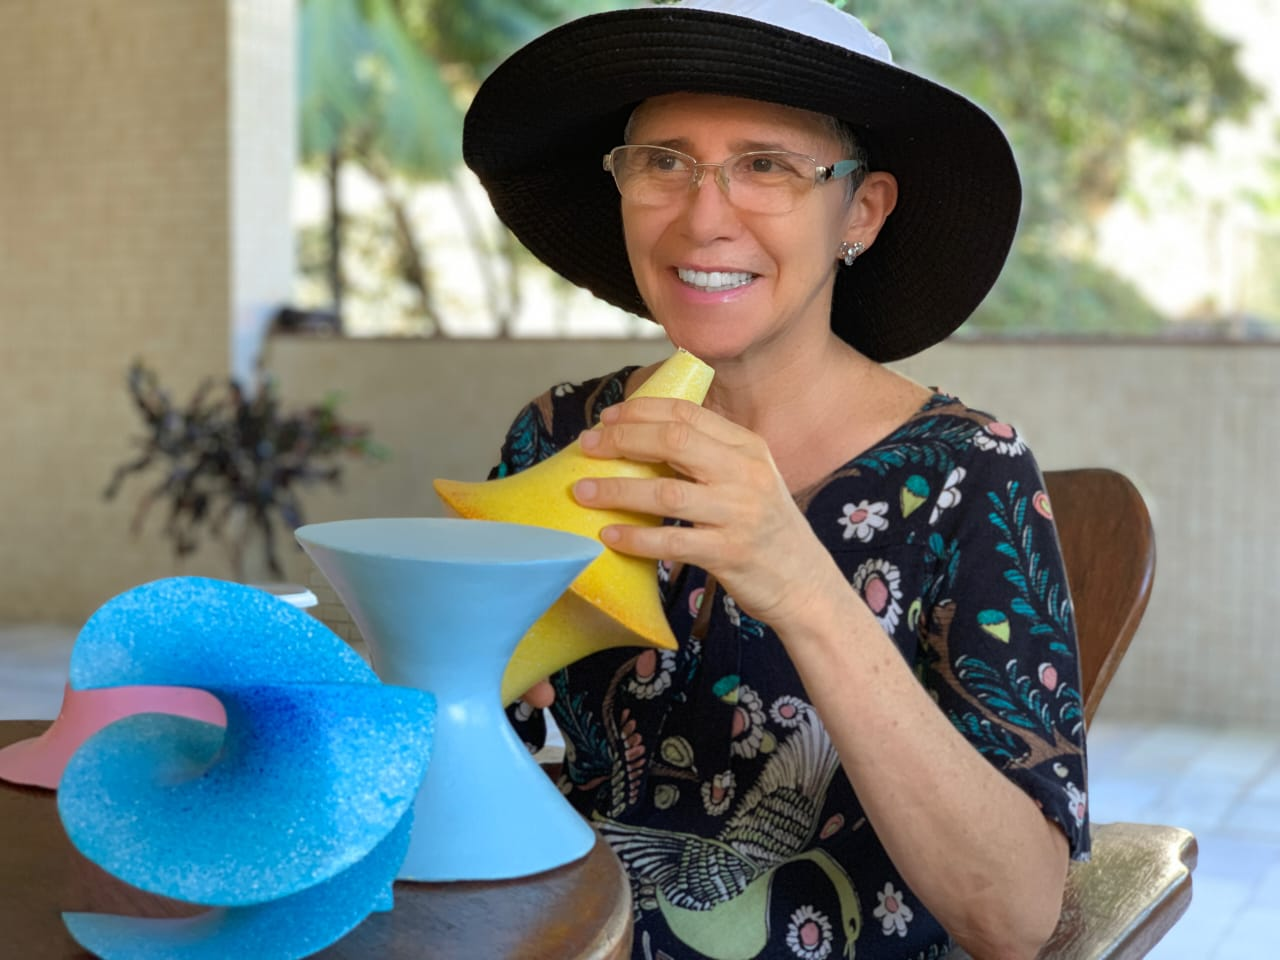
\includegraphics[width=8cm]{LEMA1.jpeg}
\caption{O sorriso diante dos modelos do LEMA.}   
\end{figure}


Ao longo de sua trajetória, a professora Lina destacou-se por sua alegria, criatividade e profundo comprometimento com o ensino da Matemática. Sua didática envolvente e seu entusiasmo contagiante tornavam suas aulas experiências marcantes, capazes de transformar a percepção que muitos estudantes tinham da disciplina. Para diversos ex-alunos, suas aulas e orientações foram decisivas para manterem-se motivados na graduação, enxergando a Matemática de forma mais humana, acessível e prazerosa.  

Um dos pilares dessa transformação foi o LEMA. Inspirado em cursos de aperfeiçoamento de professores realizados em 1992 e 1993, o Laboratório de Ensino de Matemática foi instalado em 1996, na sala 148 do  então IM-UFBA, com o nome e os recursos do Projeto “Laboratório Referencial das Licenciaturas da UFBA”, referente ao PROGRAD-1995. Com relação à área de Matemática, o citado projeto teve como principais objetivos iniciais: fortalecer a formação acadêmica dos licenciandos em Matemática, inserindo-os nas atividades de laboratório; e 
abrigar os cursos de atualização e de aperfeiçoamento destinados aos professores do Ensino Médio e Fundamental da rede pública de ensino, fortalecendo a integração da UFBA com a rede pública estadual e municipal, constituindo-se num ponto de referência para as escolas públicas. 

Em 1997, o laboratório promoveu a primeira exposição no SESC, apresentando um pequeno acervo de modelos construídos no âmbito do projeto. Nesse mesmo ano, foi desenvolvido o primeiro programa de monitoria com estudantes, que também serviu para prepará-los para atuarem como expositores já na segunda exposição, realizada em 1999. 

Miriam Mascarenhas, professora aposentada do DMAT, que também atuou na criação do laboratório, recorda com carinho desse início, em \href{https://youtu.be/-kerHGWxOvk}{[4]}: \begin{quote}\textit{A minha experiência com ela [Lina] no laboratório, surgiu desde o embrião. Ainda sonho com muitas conversas e ideias. Mas com a dedicação incansável, trabalho, estudo, pesquisa, elaboração de projetos...nasceu o LEMA. Participei de várias bienais, exposições em escolas e no IM-UFBA, com a equipe de
professores e alunos, e apesar de pouca verba, era tudo feito com muito amor, com muita alegria, e estudo. O ambiente não podia ser melhor[...]}. \end{quote}

Desde então, o laboratório consolidou-se como um espaço singular de formação docente, ensino e extensão, adotando oficialmente, em 2007, o nome “Laboratório de Ensino de Matemática e Estatística da UFBA (LEMA)”. Hoje, o LEMA conta com 3 salas no IME-UFBA: 150 (sala de estudos para monitores, bolsistas e voluntários do LEMA, compartilhada com os estudantes do PIBID), 142 (conhecida como ateliê) e a 141, que abriga o acervo atual de aproximadamente 200 modelos concretos direcionados para o ensino fundamental, médio e superior. Produzidos ao longo dos anos por estudantes e professores envolvidos em suas atividades, além da colaboração da artista plástica Fabiana Laranjeiras, esses modelos são utilizados para aulas de disciplinas do Departamento de Matemática, Estatística, Física, além de estarem disponíveis para ações junto à comunidade externa da UFBA, como feiras, exposições e oficinas.  

Prestes a completar 30 anos de existência, o LEMA já realizou inúmeras exposições em Salvador, em outras cidades da Bahia e do Brasil, e até em Angola. O laboratório também recebe com frequência a visita de estudantes de escolas e universidades, em atividades cuidadosamente organizadas pela coordenadora  do LEMA, Cristiana Valente, e pela vice-coordenadora, professora Denise Viola, do Departamento de Estatística da UFBA (DEST). A equipe atual para organização de atividades e elaboração de projetos do LEMA ainda conta com as professoras Elaís Cidely S. Malheiro (DMAT) e Lilia Costa (DEST).

\begin{figure}[htb!]
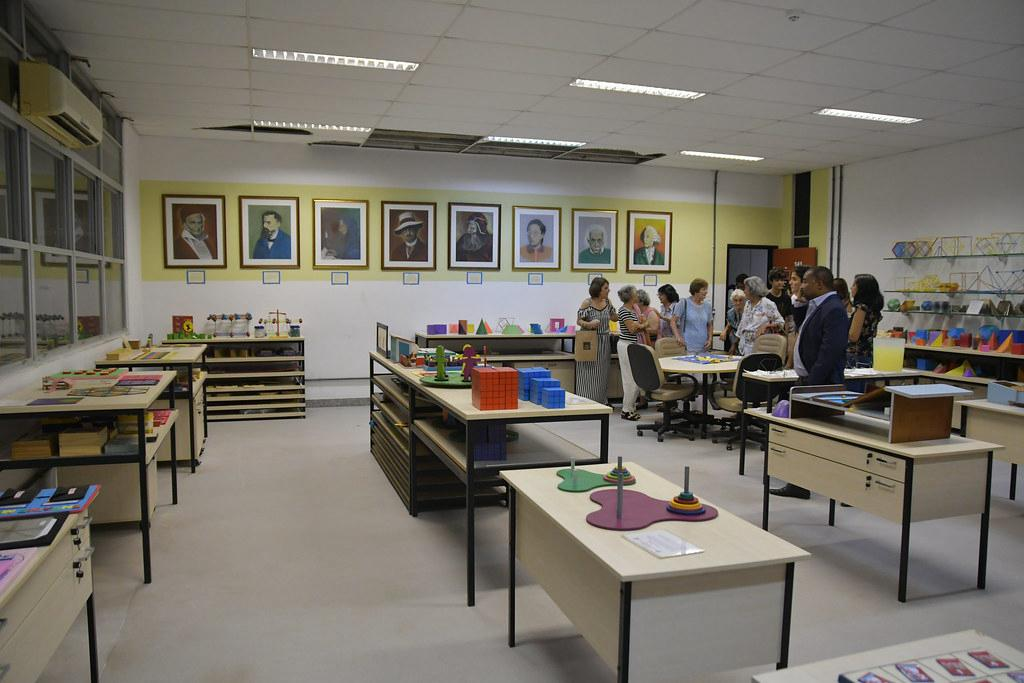
\includegraphics[width=8.7cm]{Lab.jpeg}
\caption{LEMA.}   
\end{figure}


Lina foi a mente e o coração por trás da criação do LEMA, coordenando com inteligência e sensibilidade uma equipe diversa de professores e estudantes. Sua liderança acolhedora e persistente fez do laboratório um verdadeiro berço de experiências inovadoras na formação de professores de Matemática. O egresso do DMAT, Renivaldo Sodré, hoje professor da Universidade Federal do Ceará, sintetizou o impacto dessa convivência em \href{https://youtu.be/-kerHGWxOvk}{[4]}: \begin{quote}
  \textit{A Prof. Elinalva Vergasta me ajudou a entender e olhar o mundo com um olhar geométrico e humano.
Minha história no LEMA-UFBA coincide com a minha trajetória na UFBA. Ingressei na Instituição, no
dia 31 de maio de 2004.
E, nesse mesmo dia, foi apresentado o projeto LEMA-UFBA pelas professoras Cristiana Valente e Elinalva Vergasta.
A Lina entrou na sala de recepção dos calouros com um chapéu de Sherlock na cabeça, com muito carinho e muito entusiasmo, falava e convidava a gente para participar do projeto. Nesse mesmo dia, ingressei no projeto LEMA-UFBA, “fui a orelha seca, fui a orelha gorda”, vivi intensamente o LEMA.
E o LEMA contribuiu de maneira fundamental, na minha formação profissional e pessoal.}   
\end{quote}

\begin{figure}[htb!]
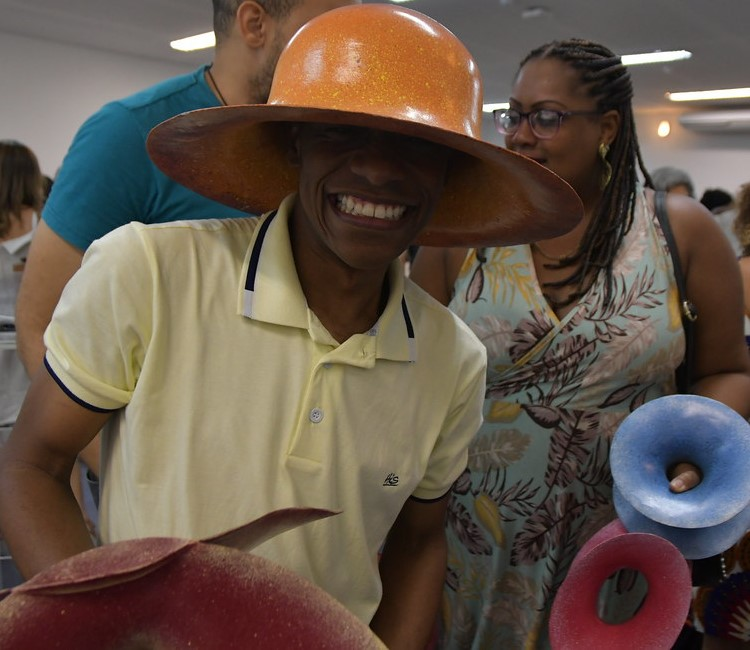
\includegraphics[width=8.7cm]{Reni.jpg}
\caption{Renivaldo com o famoso chapéu de Sherlock, na homenagem pra Lina de 2019.}   
\end{figure}


Sob sua orientação, o LEMA impactou diretamente o ensino de Matemática em toda a Bahia. Diversos ex-estudantes lembram com carinho do laboratório como uma “grande escola”, onde se aprendia não apenas conteúdos matemáticos, mas também como ensinar com criatividade, ludicidade e eficiência. Lina estava sempre presente — orientando construções, organizando exposições, viajando com os alunos para encontros científicos e cuidando para que todos se sentissem valorizados. Mesmo estudantes do bacharelado, não diretamente ligados à licenciatura, se envolviam nas atividades do laboratório, demonstrando o alcance e o apelo da proposta pedagógica que Lina cultivou. 


Durante três décadas como professora do Instituto de Matemática, Lina recebeu inúmeros reconhecimentos formais e informais por sua atuação no ensino de Matemática. Foi escolhida por diversas turmas de formandos como patronesse, paraninfa, madrinha ou “amiga da turma” — um reflexo do carinho e da gratidão que despertava em seus alunos. O seu trabalho à frente do laboratório ganhou destaque nacional, com convites para diversas oficinas e exposições, incluindo em edições da Bienal da Sociedade Brasileira de Matemática.  


Em 2018, foi aprovada em reunião da Congregação do IME, que estava, na época,  sob a direção do professor Evandro Santos, a nomeação da sala 141 do IME como "Laboratório de Ensino de Matemática e Estatística / Prof.\superau Elinalva Vergasta de Vasconcelos". Este importante reconhecimento do Instituto à principal responsável pela criação e consolidação do LEMA culminou em uma emocionante cerimônia de homenagem à Lina, organizada sob a coordenação da professora Cristiana Valente, em 2 de dezembro de 2019.

\begin{figure}[htb!]
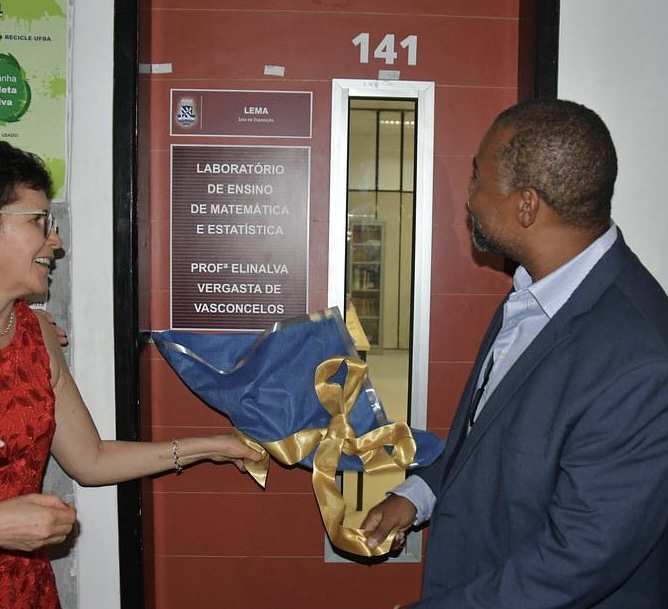
\includegraphics[width=8cm]{Evandro.jpg}
\caption{Durante homenagem 2019, com o professor Evandro.}   
\end{figure}


Quinze anos após sua aposentadoria, Lina continua influenciando na formação de alunos(as), na atuação de docentes e na vida de ex-estudantes, colegas e amigos.

Em janeiro de 2025, o projeto de extensão do DMAT "Projeto Egressos dos Cursos de Matemática da UFBA, Conectando Passado, Presente e Futuro no IME" (PECMat) promoveu uma homenagem à professora Elinalva, organizada sob a coordenação da professora Elaís Cidely.

Esta homenagem contou com uma oficina destinada a estudantes da graduação em Matemática do Instituto Federal de Educação, Ciência e Tecnologia da Bahia (IFBA - Unidade de Salvador), no dia 21 de janeiro, e uma palestra, no auditório do IME, dia 23 de janeiro, seguida da exibição de vídeo com depoimentos sobre Lina de ex-estudantes e amigos que não puderam estar presentes na ocasião, além de emocionantes relatos de participantes presentes.

A oficina intitulada `Demonstração do Teorema de Pitágoras' foi ministrada por Paulo Malta, professor do IFBA (Unidade de Porto Seguro), que também é egresso do DMAT e ex-aluno de Lina. Ao ser indagado pela organização do evento sobre ter dirigido quase 800km, de Porto Seguro a Salvador, apenas para ministrar a oficina, o professor respondeu: \begin{quote}
    \textit{Se tratando de atividade relacionada à Elinalva ou ao LEMA, pode sempre contar comigo, faço questão de participar, independente de onde eu estiver e do quanto precisar me deslocar.}
\end{quote}

Já a palestra, intitulada "Minha Vida Como Rato de Laboratório: Impactos do LEMA em Minha Trajetória Acadêmica e Pessoal", foi ministrada pelo doutorando em Matemática na UFBA e também professor do IFBA (Unidade de Salvador) Fellipe Antônio. Como evidencia o próprio título da palestra, Fellipe atuou de forma intensa no LEMA durante a sua graduação, e já como professor do IFBA, foi um dos principais responsáveis pela implementação do Laboratório de Matemática do IFBA (LEMAT). Em relato enviado aos autores, ele ressalta características marcantes em Lina:
\begin{quote}
    \textit{Quando você pergunta dela a qualquer pessoa que a conhece, certamente vão falar do carisma, da simpatia, da boa vontade e do bom humor. Inevitável não falar da criatividade, da leveza e da competência. Todos os estudantes preferiam fazer disciplina com ela e todos admiram-na profundamente. Era comum ela aconselhar seus alunos mesmo depois que deixavam de ser seus alunos. Era como mãe pra muitos: ela escutava, orientava, acolhia, puxava a orelha. Lina ensinava não apenas conteúdos e matemática, embora fizesse prioritariamente isso de forma magistral...a convivência com ela nos dava exemplo de valores como honestidade, retidão, compromisso, humildade, humanidade, dedicação, perseverança. Quando a ideia de um modelo vinha, ela tomava nota, nem sempre as coisas funcionavam de primeira, na verdade, muitos modelos do LEMA de hoje são versões melhoradas, fruto de pesquisa, esmero, dedicação e perseverança. Ainda há alguns que até hoje são ideias que ainda não tomaram forma. Hoje com o advento da cultura maker, eu vejo que Elinalva era um bom exemplo de "teto alto" e "paredes largas", ela não limitava a criatividade dos estudantes  e orientava como aproveitar o máximo. Também não dá pra falar de Elinalva sem se referir à energia canalizada à dedicação; era comum receber e-mails escritos na madrugada ou vê-la com uma listinha de coisas grande, o empenho em redigir projetos, revisar, unir pessoas diferentes em prol de um mesmo objetivo. Ela também era muito generosa: oferecia sempre algum lanche, alguma fruta, perguntava se precisávamos de carona, ficava preocupada com nossa segurança quando inventávamos de sair tarde... Elinalva é para mim um grande exemplo: de família, de mulher, de professora, de ser humano, de liderança, de criatividade, de estudo.}
\end{quote}
A homenagem foi para Lina, mas a comunidade do IME foi presenteada com a presença da própria professora, que estava acompanhada do seu marido Dioni e sua cunhada Ionevera Vasconcelos. Entre os participantes, além de atuais estudantes e docentes do DMAT, também estiveram presentes diversos professores aposentados do DMAT. Este encontro de gerações, impulsionado pela potente e inesquecível atuação da professora Elinalva no DMAT, ressalta como o legado de Lina segue vivo — nos gestos, nas memórias e nas escolhas de quem teve o privilégio de aprender com ela. Sua presença serena e afetuosa foi mais do que simbólica: foi a confirmação de que verdadeiros educadores continuam ensinando, mesmo depois da sala de aula.

\begin{figure}[htb!]
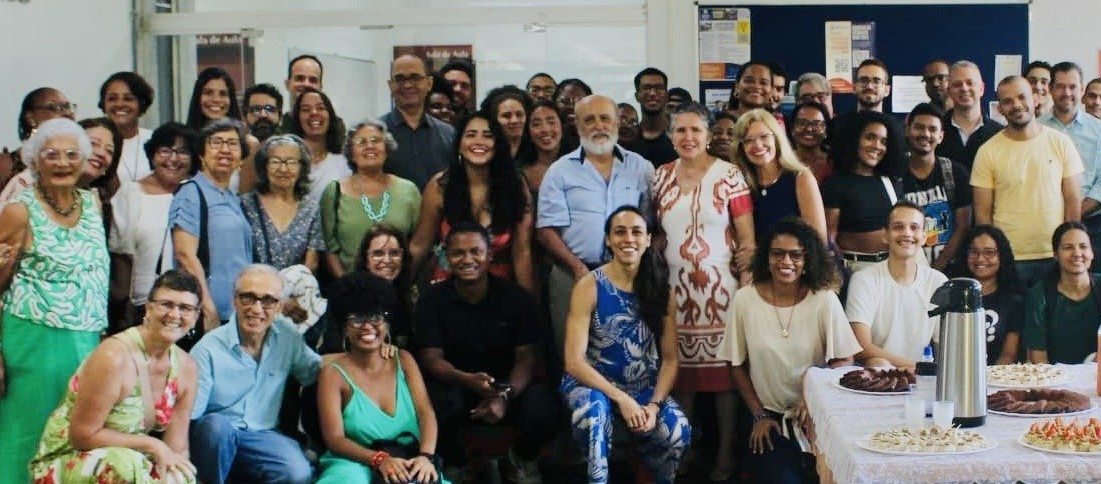
\includegraphics[width=8.7cm]{2025.jpg}
\caption{Homenagem 2025, promovida pelo projeto de extensão PECMat.}   
\end{figure}

%Para ela, ensinar era mais do que transmitir conteúdos — era abrir caminhos de compreensão e encantamento. Sua forma de pensar e ensinar matemática também expressava esse traço estético e afetivo: a beleza do raciocínio claro, da organização elegante das ideias, da curiosidade em movimento. O LEMA é, sem dúvida, uma das expressões mais marcantes do seu legado — um espaço construído com carinho, competência e visão pedagógica, que formou não apenas professores, mas também cidadãos comprometidos com a educação matemática, que carregam um pouco de sua forma de ver e viver a Matemática: com afeto, competência e...arte. 


\section{Relatos sobre Lina}

Os depoimentos abaixo de ex-alunos, colegas e amigos foram gravados para as homenagens à Lina realizadas em dezembro de 2019 e janeiro de 2025, ou enviados aos autores do presente artigo.

Jamille Vilas Bôas, professora do IFBA: \begin{quote}
\textit{Eu me recordo muito bem, no primeiro dia da graduação, em um dado momento, foi convidado a coordenadora do Laboratório de Matemática da UFBA pra gente conhecer. E chega a professora Elinalva, com a representação de um quadrado e quatro triângulos retângulos na mão, para ilustrar o Teorema de Pitágoras. E fez tudo aquilo parecer uma mágica. Me encantou muito aquela possibilidade. E, a partir de então, eu não saí do lado dela. Foram muitos projetos,  muitas exposições, muitas atividades no
Laboratório de Matemática da UFBA que eu participei.
E o LEMA é isso, e a professora Elinalva também, representa a minha trajetória dentro da UFBA. Fico muito feliz por poder falar isso para ela. E emocionada, porque inspirou também o meu mestrado sobre a
participação de alunos utilizando materiais manipulados em sala de aula no ensino da matemática. O meu doutorado teve a ver com isso também.}
\end{quote}

Manuela Souza, professora da UFBA: \begin{quote} \textit{Lina fez parte da minha formação, tanto nas atividades e exposições do LEMA, que durou a época do Bacharelado e Mestrado, como também sendo minha professora de Geometria Diferencial. Meu primeiro contato com essa área aconteceu através do modelos de superfícies mínimas do LEMA, logo no primeiro ano de graduação. Lina influenciou, certamente, muito da minha prática docente hoje e é uma referência de como aliar ensino e pesquisa em Matemática, porque, sim, o LEMA-UFBA é, também, sobre pesquisa em Matemática.} \end{quote}

Belmiro Galo, professor da Rensselaer Polytechnic Institute(EUA): \begin{quote} \textit{Nossa querida professora Lina. Lina, muito obrigado por todo o apoio que você deu no meu tempo
de UFBA com cálculo IV. E também como seu monitor versátil do LEMA. Nunca um monitor oficial, mas
sempre estava ali quebrando um galho. Lembro de um momento marcante quando tinha acabado de tirar
minha habilitação, não sabia dirigir direito, e véspera de uma exposição que a gente tinha no
departamento, você me deu a chave do seu carro e falou "vai lá no Instituto de Física, pega lá os
materiais que estão lá, estamos precisando e, não tenho tempo...". Você estava na correria, meu Deus, meu pé tremia para dirigir seu carro. Acho que foi a primeira vez que dirigi um carro fora da autoescola. Foi o seu carro, [você] só me deu a chave, e falou "vai", e confiou em mim. Deu tudo certo, não dei nenhum arranhão, e passou. Mas sua paixão pela matemática, pelo departamento e pela educação foi contagiante e estou aqui hoje sendo professor também da universidade, aqui no exterior, e muito feliz por toda a sua contribuição. Obrigadão Lina}.\end{quote}

Sílvia Veloso, professora aposentada do DMAT: \begin{quote}
\textit{Fui contemporânea de Lina no curso de matemática e depois nos tornamos colegas de trabalho como
professores do Instituto de Matemática da UFBA. Nossos caminhos convergiram em alguns projetos e o maior deles foi o LEMA, criado e idealizado por
Lina, e eu sempre brincava: ela é a cabeça do laboratório e nós somos os membros. Ela conseguiu formar
uma equipe muito boa e agregou muitos alunos de uma forma assim muito harmoniosa.
Isso era um marco de Lina. Ela tinha essa capacidade além de muitas outras características muito
marcantes. Ela era uma pessoa inteligente, muito estudiosa, esforçada, com a capacidade incrível de
coordenação, de manter todo mundo em paz, em equilíbrio, dedicado, se dedicando, sempre sorrindo.
Não existia dificuldade nem tempo ruim para a Lina. Eu lhe quero muito bem, foi muito bom ter
trabalhado com você. O tempo é curto para ele dizer qualquer coisa mais, mas desejo tudo de bom para
você, Lina. E você é muito especial para mim e na minha caminhada, na minha construção como
profissional. Um beijo no coração.}
\end{quote} 

Márcio Peixoto, vizinho de Lina:
\begin{quote} \textit{Falar de Lina é falar de PORTAS ABERTAS! Sim, não só pelo fato de termos sido vizinhos por 26 anos, as portas da sua casa viviam sempre abertas para os amigos, e para mim que sempre fui quietinho senão encontrasse aberta por qualquer razão, eu pulava a varanda, mas mais importante que isso, Lina nos abriu portas para um conhecimento valioso... foi ela quem me apresentou ao primeiro computador, quantas vezes me levou ao teatro, me encorajou a encenar peças, a me tornar síndico mirim do nosso condomínio, as idas à praia (na inesquecível Belina azul) quantos filmes vimos, quantas pizzas na Ilforno, quantas risadas demos juntos, quantas caronas, quantas lições...
Homenagear Lina é olhar pra trás e abraçar uma fase muito especial da minha vida... agradeço por ter me permitido beber dessa fonte de conhecimento sem nem sequer me dar conta, naquela época, do quão importante isso representaria para mim nos dias atuais! Obrigado, querida vizinha! Parabéns por essa homenagem.} \end{quote}

Fabiana Laranjeiras, artista plástica:
\begin{quote} \textit{Elinava em minha vida, teve uma participação grandiosa como educadora. Lina me conheceu no fim do ano de 1996, quando eu era estudante de Belas Artes e ela queria desenvolver as superfícies dos modelos das Quádricas em resina. Como o trabalho com a resina não deu muito certo, desenvolvemos as pesquisas com a técnica de Papietã, que até hoje está sendo trabalhada com os alunos das disciplinas do LEMA.
Eu, quando estudante, aprendi muito com a organização de textos, arquivos de imagens e vídeos, registros fotográficos e de vídeos nas visitas e exposições do LEMA, o que me trouxe muito conhecimento técnico computacional proposto por Lina. E uma das coisas mais importantes além do apoio técnico artístico na construção e restauração dos modelos que até hoje estão sendo expostos no LEMA-UFBA, foi a participação como ilustradora (vetorizadora) dos desenhos dos 2 livros escritos pelas professoras que compunham o quadro de fundadoras do nosso querido laboratório.
O resumo da minha passagem pelo LEMA-UFBA é GRATIDÃO!} \end{quote}

Cristiana Valente, professora da UFBA e atual coordenadora do LEMA:
\begin{quote} \textit{Falar sobre Elinalva, uma querida amiga, pseudo-mãe matemática e "ídola", é muito fácil! O difícil é lembrar de toda a lista de tudo que tenho que relatar sobre ela, mas vamos lá...
Meu contato inicial com Elinalva foi como aluna de Topologia e nas suas aulas ficava
encantada como ela apresentava esses conteúdos matemáticos, avançados para graduação,
de uma forma tão simples e natural. [...].
Depois recebi seu apoio para fazer mestrado na USP e quando precisei voltar para Salvador,
ela me enviou material de Geometria Analítica para fazer seleção para professor substituto no
antigo Instituto de Matemática, atualmente IME. Depois seu apoio continua no processo de
preparação para o concurso e, então, com a aprovação, viramos colegas! Nosso convívio foi aumentando e a amizade cada vez mais, por conta de vários projetos que trabalhamos juntas e também pelo convívio social com amigos comuns. Mas só depois que entrei no LEMA que pude realmente acompanhar seu trabalho de perto. Além de participar de exposições, algumas
em viagem, projetos com outros professores e alunos, ela me convidou para apresentar palestras, oficinas de construção de modelos, etc. Isto é, me deu oportunidades de muitos
trabalhos que nunca tinha realizado.
Depois ela me convidou para coordenar exposições e com isso, sem eu perceber(rsrsrs) foi
me preparando para eu coordenar o LEMA, quando se aposentasse.
Elinalva foi uma profissional completa, porque atuava no ensino, pesquisa e extensão, além de
trabalhar na parte administrativa da UFBA.
Elinalva era assim: as ideias iam surgindo e ela ia convidando as pessoas, professores e/ou
alunos, para estudar Matemática, produzir novos materiais, como por exemplo modelos concretos, etc, com o objetivo de facilitar o aprendizado em Matemática. Tudo isso sem impor
ideias, respeitando o limite da cada um.
Outra coisa que admiro muito é como Elinalva fez com que o LEMA crescesse, conseguindo mais espaço em salas, mobiliário, aumentando o acervo dos modelos, organizando exposições em
vários estados do nosso país, tornando o laboratório reconhecido nacionalmente.
E o mais incrível foi que, apesar da fama, Elinalva nunca se colocou em evidência, nem fazia
propaganda de ser a fundadora e coordenadora do LEMA.
Gostaria também de destacar a maneira com que Elinalva procurava resolver os problemas que surgiram, sempre com firmeza, mas de forma leve, sem confrontar as pessoas de forma
ríspida, procurando o diálogo.
De todos os projetos, o LEMA é o que mais trabalhamos juntas e que continua até esse momento com o trabalho da elaboração de mais um livro sobre construção de modelos concretos, junto com nossas queridas companheiras Christina, Graça Passos, Verlane,
Ritinha e a grande contribuição da saudosa Nalvinha.
Por esses motivos (e outros que provavelmente vão terminar surgindo quando eu reler esse
texto), Elinalva, além de amiga maravilhosa e profissional excepcional, é um exemplo de ser
humano especial... humilde, respeitadora, amorosa. E tenho certeza que me tornei uma
matemática e uma pessoa melhor por causa dela!} \end{quote}

\section{Lina, presença que permanece}

Hoje, Lina segue colhendo o carinho de todos que a admiram, cercada pela família, amigos e pelas alegrias que semeou ao longo do caminho. Nas visitas ao IME, o sorriso presente segue despertando abraços cheios de carinho e gratidão. Sua presença é sempre uma celebração — da matemática, da vida e da beleza de ensinar com paixão.

\begin{figure}[htb!]
\includegraphics[width=8cm]{Família.jpeg}
\caption{Família.}   
\end{figure}

Neste dezembro de 2025, Lina completará 70 anos de uma vida marcada pelo entusiasmo, pela leveza e por uma dedicação profunda ao ensino da Matemática. Para ela, ensinar era mais do que transmitir conteúdos — era abrir caminhos de compreensão e encantamento. Sua forma de pensar e ensinar matemática também expressava esse traço estético e afetivo: o raciocínio claro, a organização das ideias, a curiosidade em movimento. O LEMA é, sem dúvida, uma das expressões mais marcantes do seu legado — um espaço construído com carinho, competência e visão pedagógica, que formou não apenas professores, mas também cidadãos comprometidos com a Educação Matemática, que carregam um pouco de sua forma de ver e viver a Matemática: com afeto, competência e... arte.

\vfill

\nocite{*}
\bibliography{biografia}

\pagebreak

\begin{figure}[htb!]
\includegraphics[width=8cm]{Última.jpeg}
\caption{Afeto, Matemática e Arte.}   
\end{figure}


\pagebreak


% Mini bios 
% Seja informal e divertido
% Prefira fotos com fundo branco
\begin{wrapfigure}{L}{2.7cm}
	\centering
	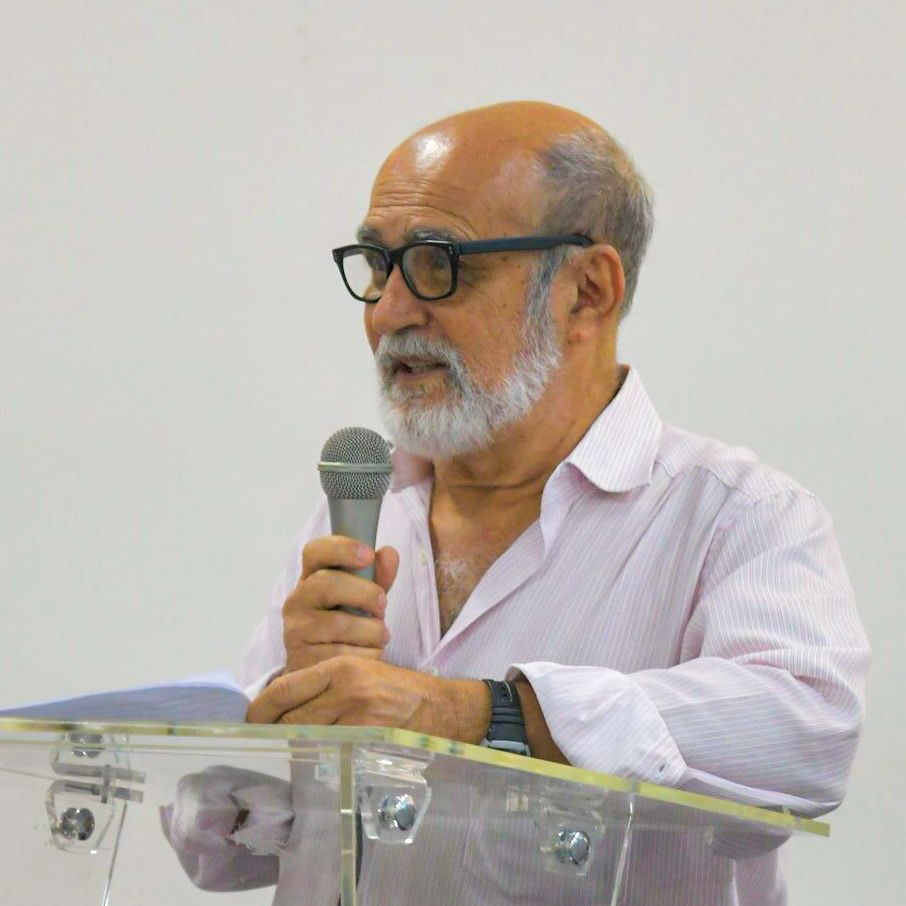
\includegraphics[width=3cm]{Dioni.jpg}
\end{wrapfigure}\noindent
Dionicarlos Soares de Vasconcelos foi professor de Física do Instituto de Física da UFBA de 1976 a 2010 e da UNIFACS após a aposentadoria por 4 anos até 2017. Fez graduação e Mestrado na UFBA e doutorado no CBPF, Rio de janeiro. Foi diretor do Instituto de Física, chefe do Departamento de Física do Estado Sólido, assessor de Informática e diretor do CPD da UFBA na gestão do Reitor Felippe Serpa. Trabalhou em pesquisa na área de Difração de Raios-X e Estruturas Incomensuráveis. Orientou muitos alunos em Iniciação Científica e Mestrado.


\vspace{2cm}
\begin{wrapfigure}{L}{2.7cm}
	\vspace{-10pt}
	\centering
	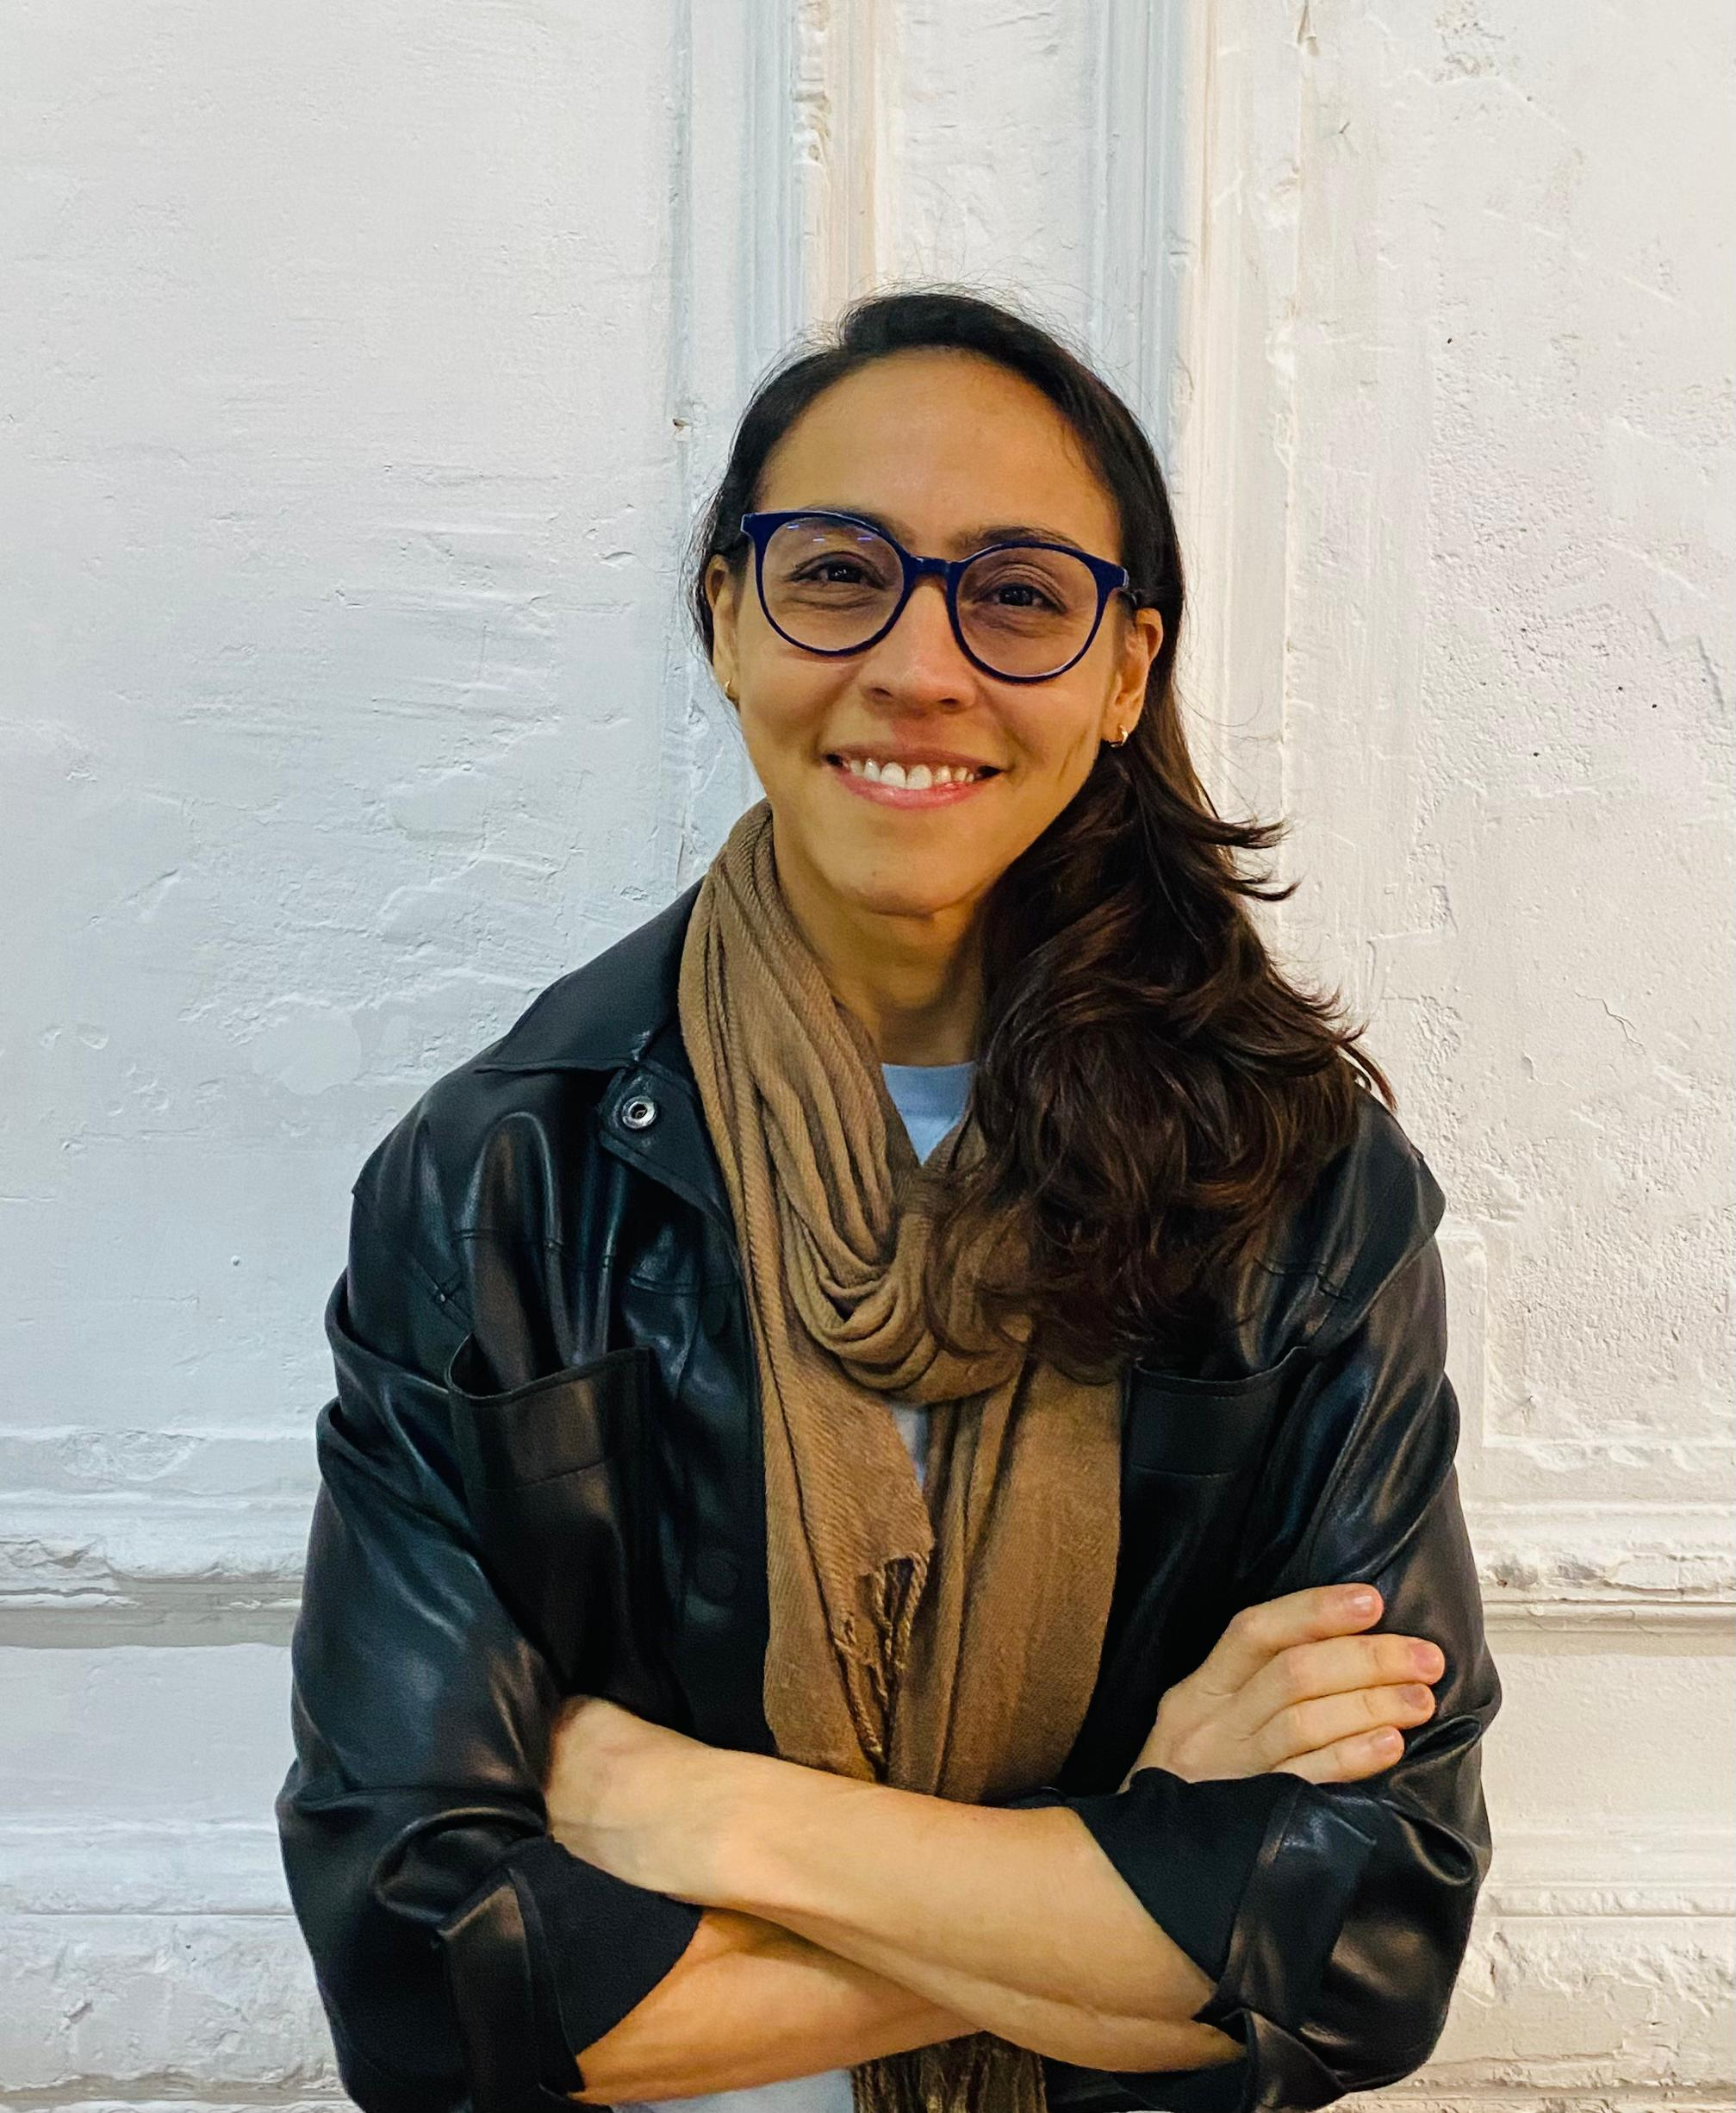
\includegraphics[width=3cm]{Elais.jpeg}
\end{wrapfigure}\noindent
Elaís Cidely S. Malheiro é baiana, nascida na cidade de Macaúbas. Possui graduação e mestrado em matemática pela UFBA, doutorado em matemática pelo IMPA e, desde 2015, é professora do IME-UFBA. Sua área de pesquisa é Sistemas Dinâmicos, com ênfase em Teoria Ergódica. Atualmente, é coordenadora local do PICME-UFBA e vice-coordenadora institucional do PROFMAT-UFBA. Além disso, coordena o projeto de extensão "Projeto Egressos dos Cursos de Matemática da UFBA, Conectando Passado, Presente e Futuro no IME"(PECMat) e atua em outros projetos de extensão, como o "Treinamento Olímpico de Matemática da UFBA"(TOM). Na adolescência,  tocou bateria em uma banda do colégio. Durante o doutorado, tocava alfaia em um grupo carioca de maracatu. Mas desde 2021, tem o CrossFit como parte indispensável da sua rotina.


\end{document}
